\chapter[Study of PLL IC CD4046]{Study of PLL IC CD4046}

\section*{AIM}

To study the characteristics of PLL IC CD4046 and find its lock range and capture range.
\section*{THEORY}

PLL is basically a closed loop electronic circuit designed to lock or synchronize the output frequency and phase to the frequency and phase of the input signal for a given range. Internal block diagram of the IC CD4046 is given in the figure \ref{PLLBLOCK}.
\begin{figure}
    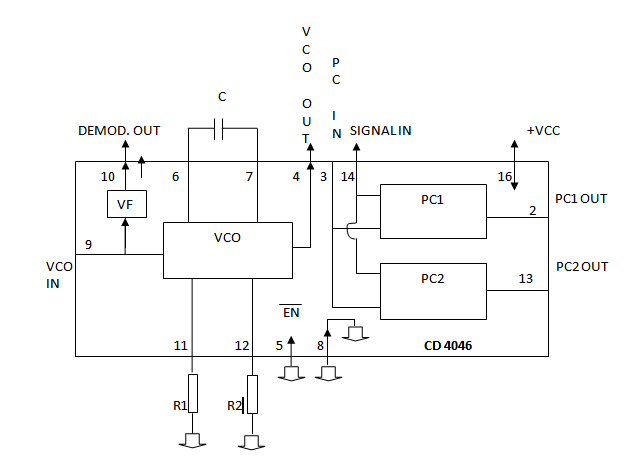
\includegraphics[width=\textwidth, height=8cm]{PLLBLOCK.png}
    \caption{Internal block Diagram of IC CD4046}
    \label{PLLBLOCK}
\end{figure}

\paragraph{}


It consists of a  linear voltage controlled oscilator (VCO) and two phase comparators. The two phase comparators have a common signal input terminal and a common comparator input terminals. The signal input terminal can be directly coupled for large input signal( upto $V_{CC}$) or capacitively coupled for small input signals (less than $\frac{	V_{CC}}{2}$). PC1 uses an XOR gate internally. Within the capture range, the output pulse width vary with the frequency difference between the signal input and the comparator input frequencies. Output amplitude is $V_{CC}$. PC1 gives a digital error signal tye pulse width of which depends on the phase difference between inputs. 

\paragraph{}Between the signal input frequency and the comparator input frequency, it may synchronise on to the signal frequencies that are close to VCo central frequency , $f_0$
or its harmonics.  PC2 is an edge triggered flip-flop circuit and its output is also proportional to the phase difference between two input frequencies. 

\paragraph{} The linear VCO produces an output frequency (pulses) whose amplitude depends on $V_{CC}$ only,  and the frequency depends on the the control voltage $V_C$ to be given to the VCO input terminal (VCOin) and resistors $R_1$ and $R_2$ and the capacitor C to be connected externally. This signal is obtained at VCOout terminal of the IC. The VCO sensitivity\footnote{oscillating voltage proportional to control voltage} is determined by $R_1$  and C and offset frequency\footnote{Frequency output at $V_C$=0} is determined by $R_1$  and C.

\paragraph{} A voltage follower is internally connected to the to the VCO input, the output of which is givena s demodulated output terminal of the IC. A pull down resistor (greater than 10 $k\Omega$) must be connected from the demodulated output terminal  to the ground. The output is taken across this resistor. For proper operation of the IC, the INHIBIT(/STROBE/ENABLE) terminal must be grounded.

The free running frequency $f_0$ is given by 
\begin{equation}
\label{f0}
f_{VCO}=\frac{0.16\ ( \frac{V_{CC}}{2} )}{R_1.C}+\frac{1}{R_2.C}
\end{equation}

\paragraph{Capture Range and Lock Range}

There are two range of frequencies that can be defined for a PLL for which the PLL output frequency can maintain synchronization with a range of input fequencies.  Within the capture range $f_c$ of PLL the output frequency will always maintain synchronization with the input signal frequency unconditionally whether the input frequency is increasing or decreasing. Within the lock range ($f_L$) of PLL the output frequency maintains synchronization with the input signal frequency with some condition. Within the lock range, towards the lower range the output mantains synchronization only when the frequency is increasing and towards the upper range of input frequencies output maintains synchronization only when the frequency is decreasing.

\section*{DESIGN}

CD 4046 can be used either as a VCo or as a phase comparator. To get the PLL operation the input signal must be given to the signal input terminal, the phase comparator input must be given from the VCOout terminal and the VCO input from the phase comparator 1 or 2 throgh a powpass filter. 

Select centre frequency =4 kHz and offset frequency =1 khz. 

\begin{equation}
f_0=\frac{0.16(\frac{V_{CC}}{2})}{R_1 C}=4 kHz
\end{equation}
Select,
\begin{equation}
C=0.01 \mu F, \therefore R_1=10k \Omega
\end{equation}

\begin{equation}
f_0= \frac{1}{R_2 C}=1 kHz
\end{equation}

Select,
\begin{equation}
C=0.01 \mu F, \therefore R_2=100k \Omega
\end{equation}

Select a lowpass filter with $R_f=10k\Omega$ and $C_f=1 \mu F$.
\section*{CIRCUIT DIAGRAM}
\begin{figure}
    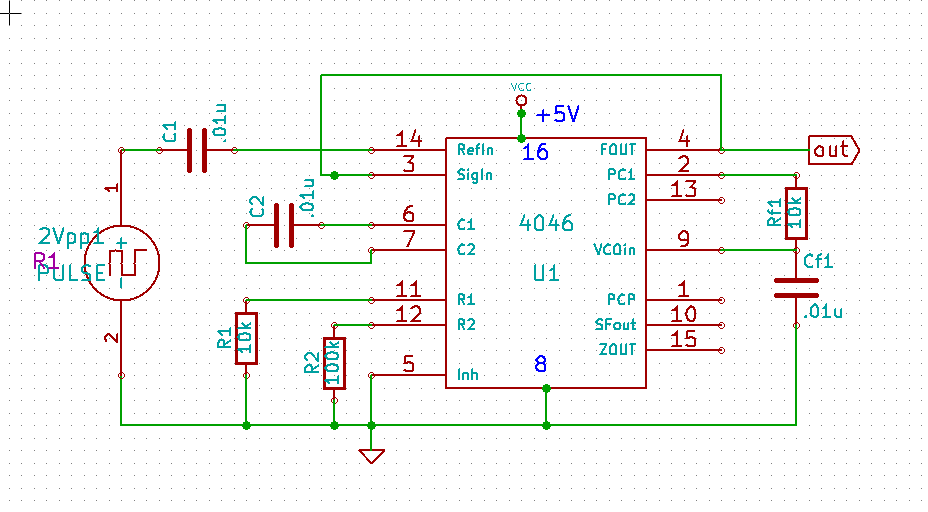
\includegraphics[width=\textwidth, height=8cm]{pllckt.png}
    \caption{Circuit Diagram to determine lock range and capture range}
    \label{pllckt}
\end{figure}


The circuit diagram as per the above design is shown in Figure 
\ref{pllckt}.

\section*{PROCEDURE}
\begin{enumerate}
\item
GND the input terminal (pin-14)
\item
Connect a CRO at the output (pin-4). The VCO output frequency will be around 5 kHz.
\item
Then remove the GND and give the input signal from the function generator throgh a capacitor and vary the input frequency at constsnt amplitude $\le 2.5 V_{pp}$.
\item
Find the frequencies $f_1, f_2, f_3$ and $f_4$.  Find $f_1$ and $f_2$ while increaing the frequency and $f_3$ and $f_4$ while the frequency is deareasing.
\item
Capture range $f_c= f_3-f_1$ and Lock range $f_L= f_2-f_4$
\end{enumerate}

\section*{RESULTS}

Studied the characteristics of PLL IC. Determined its lock range and capture range.

$f_c \approx 1.1 khz$ and $f_L \approx 7 khz$


